\documentclass{article}
\usepackage[utf8]{inputenc}
\usepackage{subfig}
\usepackage{amsmath}

\usepackage{graphicx}
\usepackage[legalpaper, portrait, margin=0.5cm]{geometry}

\thispagestyle{empty}
\renewcommand{\thesubfigure}{\roman{subfigure}}
\begin{document}

\begin{figure}[h]
        \centering
        \subfloat[3D sample rendering]{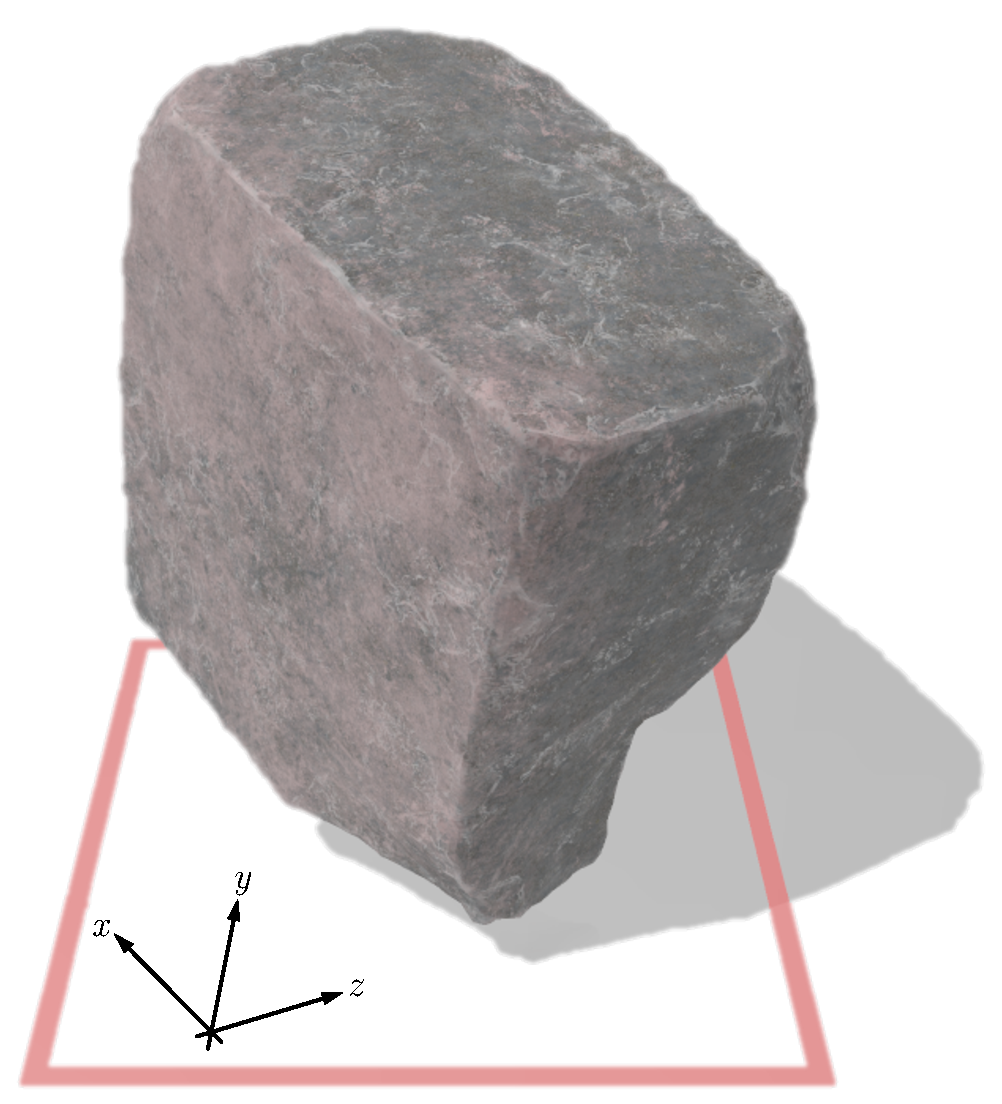
\includegraphics[height=4.6cm]{figures/ch02/3d_rendering.pdf}}\hspace{1cm}
        \subfloat[isometric view]{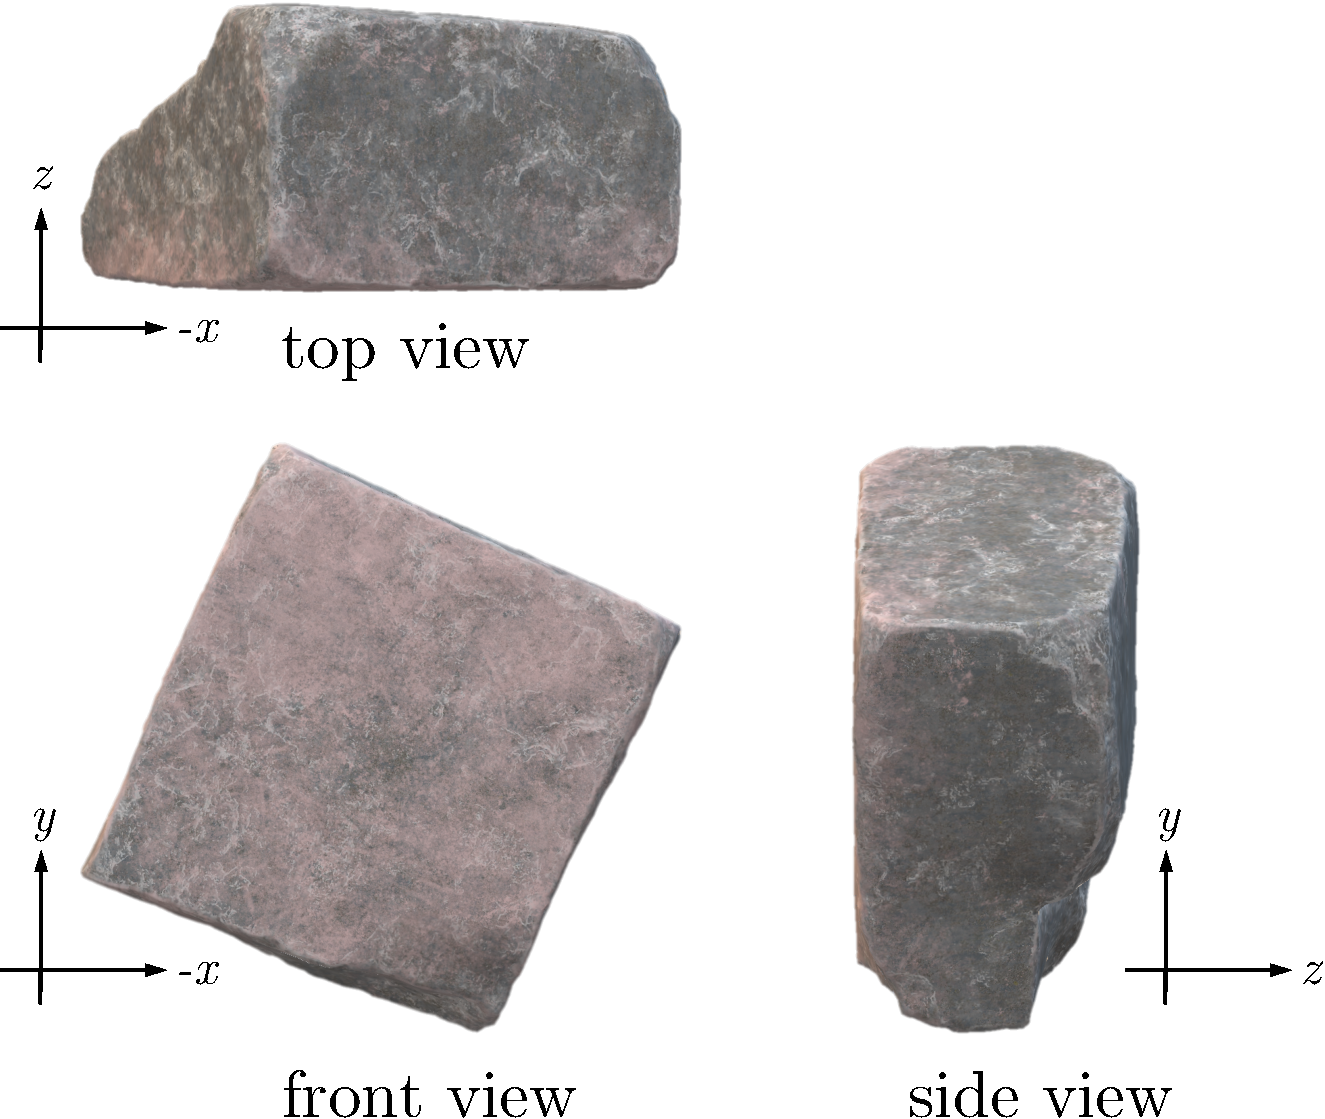
\includegraphics[height=4.6cm]{figures/ch02/isometric.pdf}}\\
        \caption*{(a) sample description}\setcounter{subfigure}{0}
        % \subfloat[]{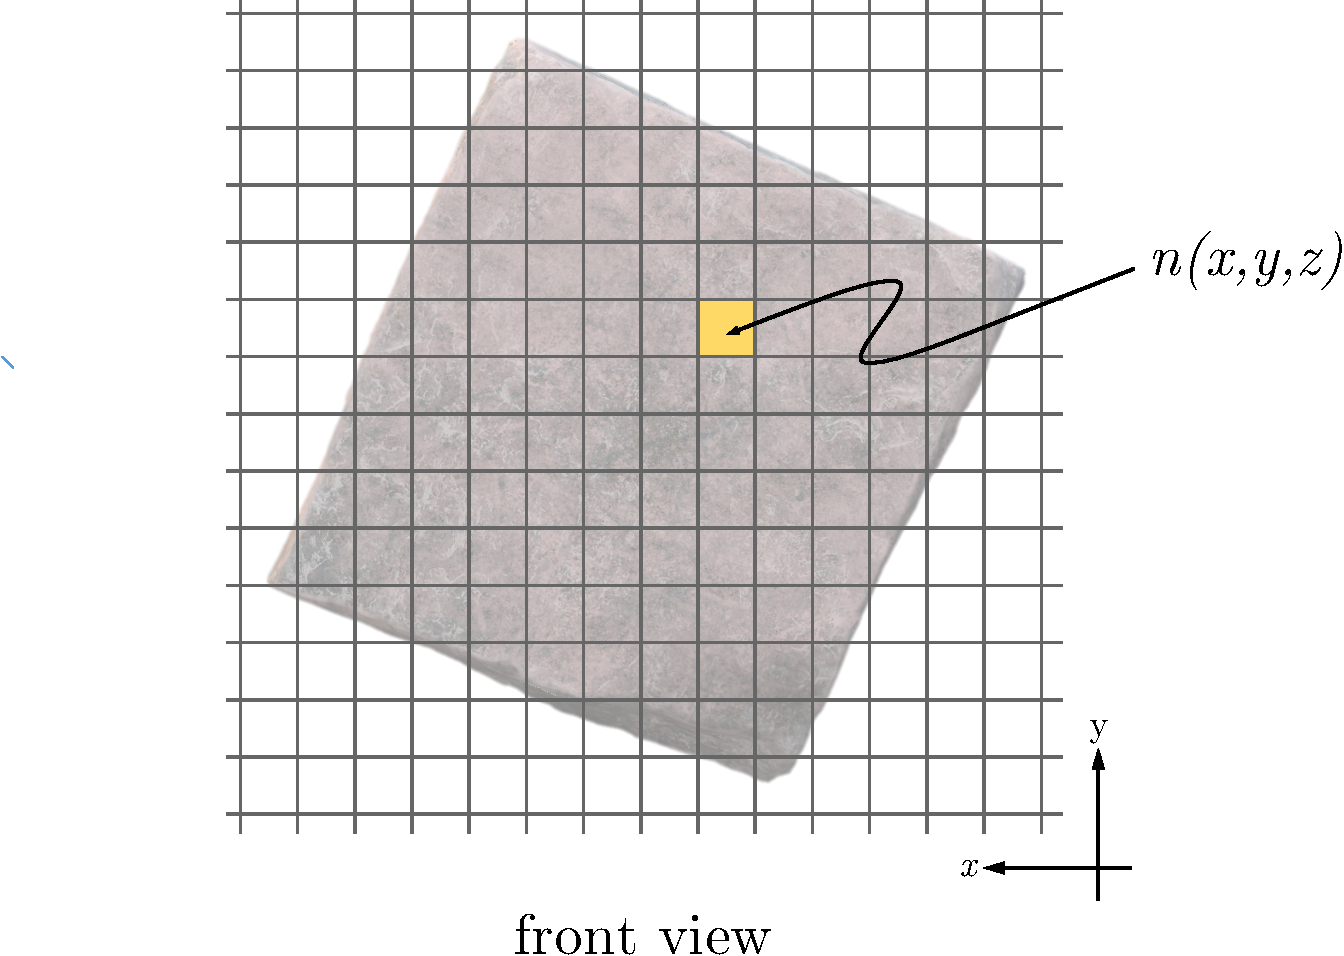
\includegraphics[height=4.2cm]{figures/ch02/thin_00.pdf}}\\
        % \caption*{index of refraction distribution}\setcounter{subfigure}{0}
        \subfloat[]{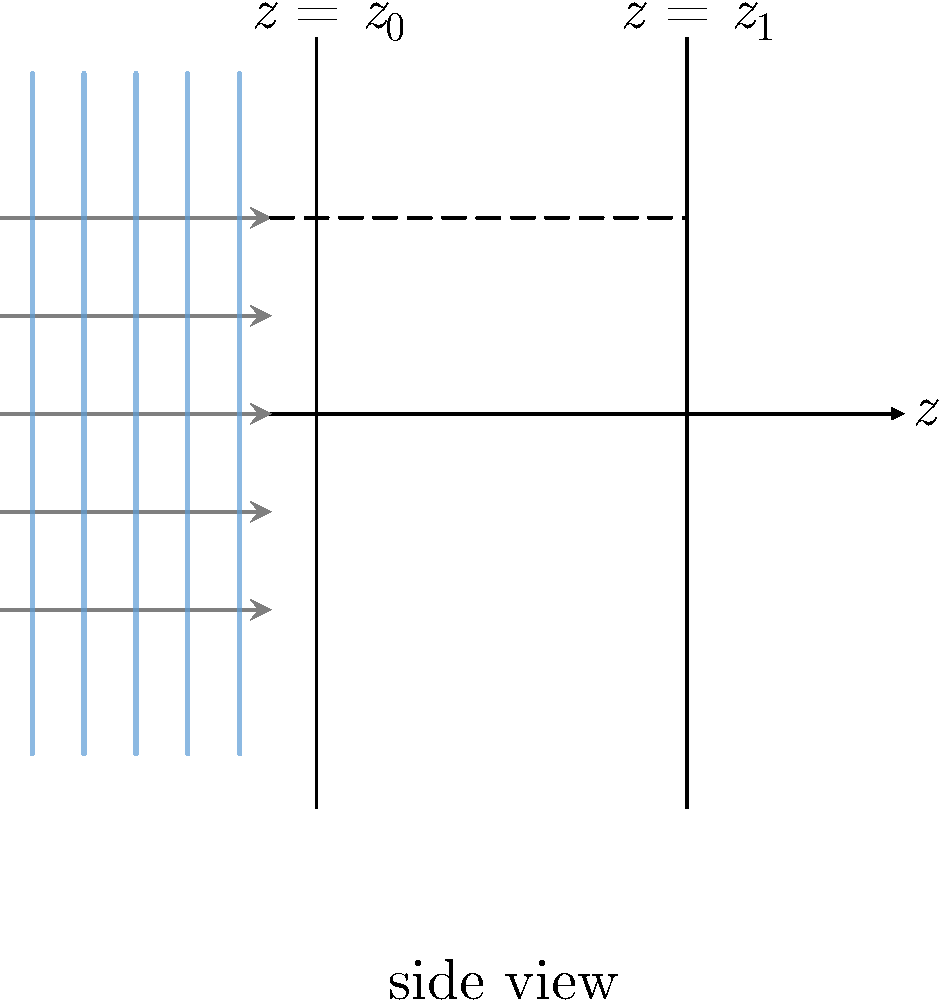
\includegraphics[height=4.6cm]{figures/ch02/thin_01.pdf}}\hspace{0.5cm}
        \subfloat[]{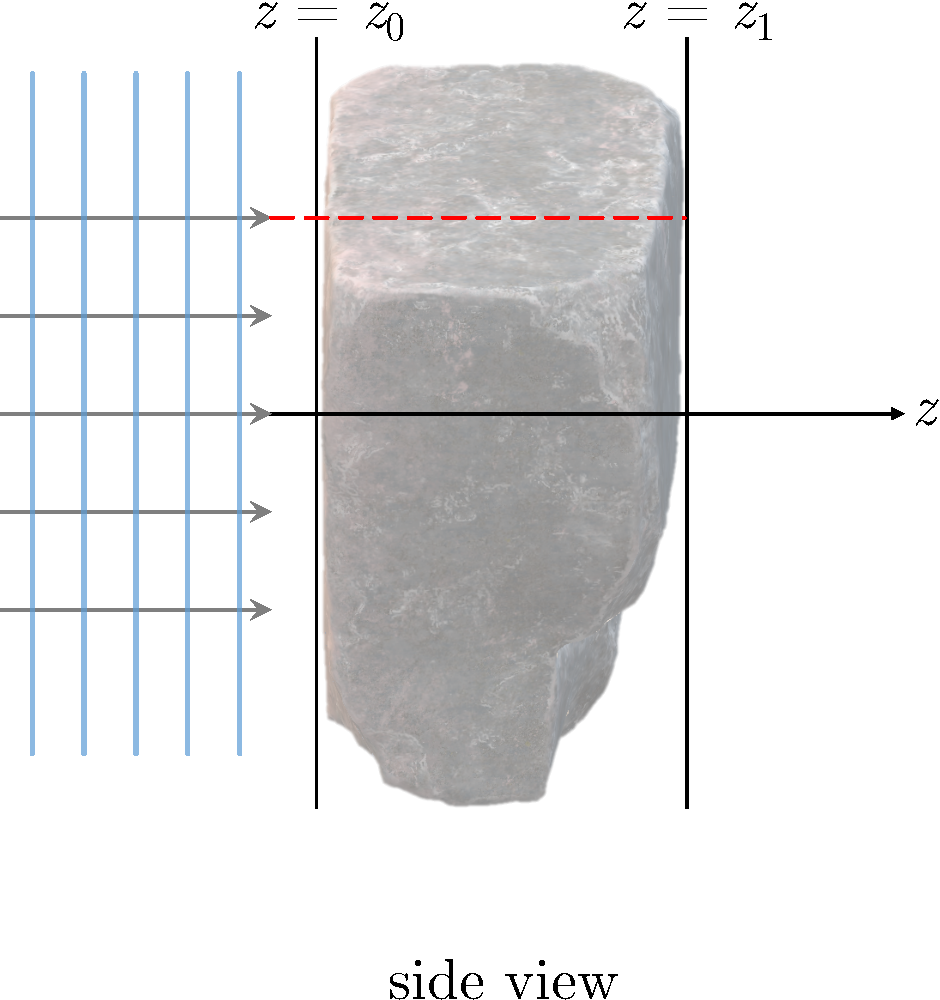
\includegraphics[height=4.6cm]{figures/ch02/thin_02.pdf}}\hspace{0.5cm}
        \subfloat[]{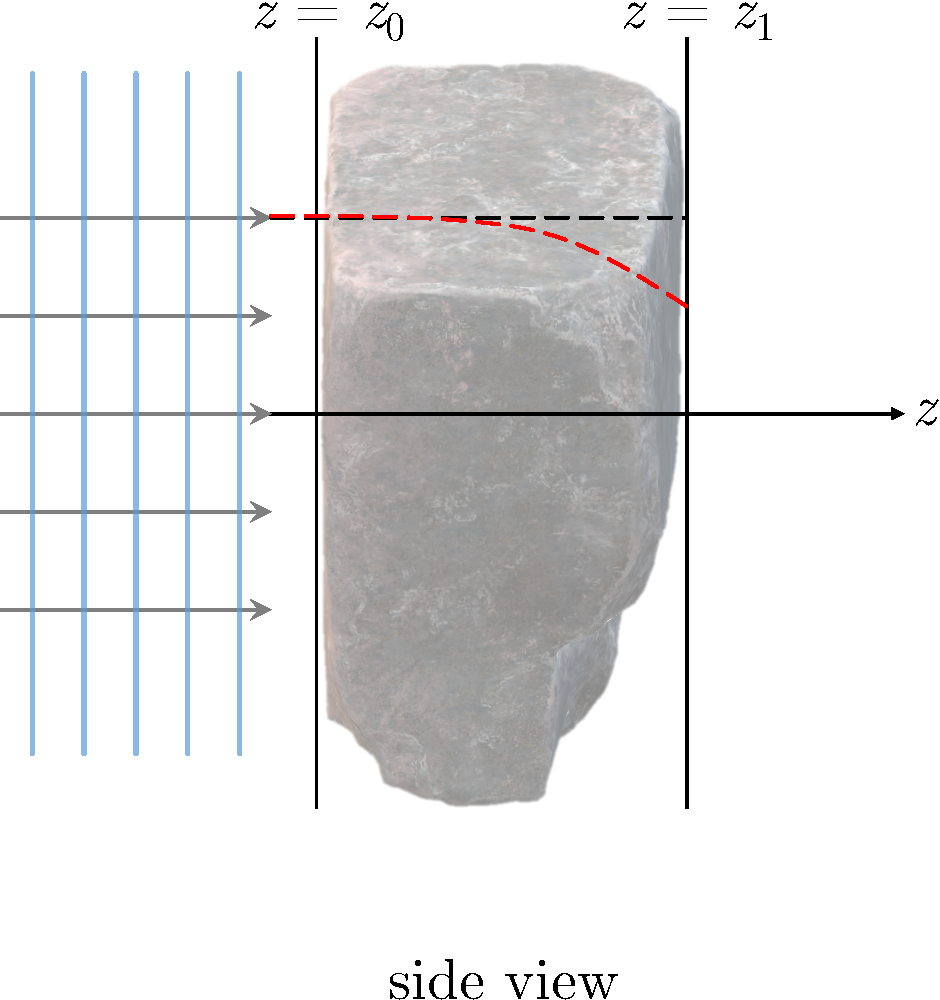
\includegraphics[height=4.6cm]{figures/ch02/thin_04.pdf}}\hspace{0.5cm}
        \subfloat[]{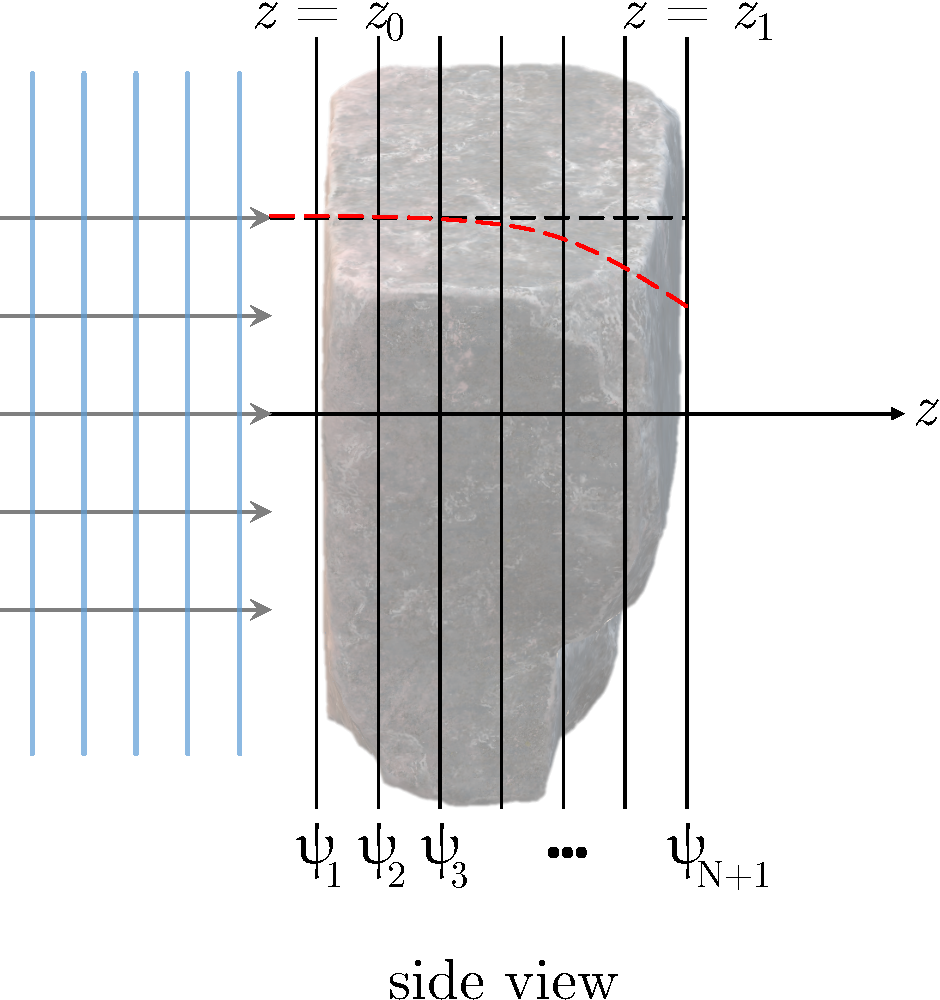
\includegraphics[height=4.6cm]{figures/ch02/thin_03.pdf}}\hspace{0.5cm}\\
        \caption*{(b) transmission element representation}\setcounter{subfigure}{0}

        % \subfloat[$\epsilon_{e}\ll\epsilon_{u}$]{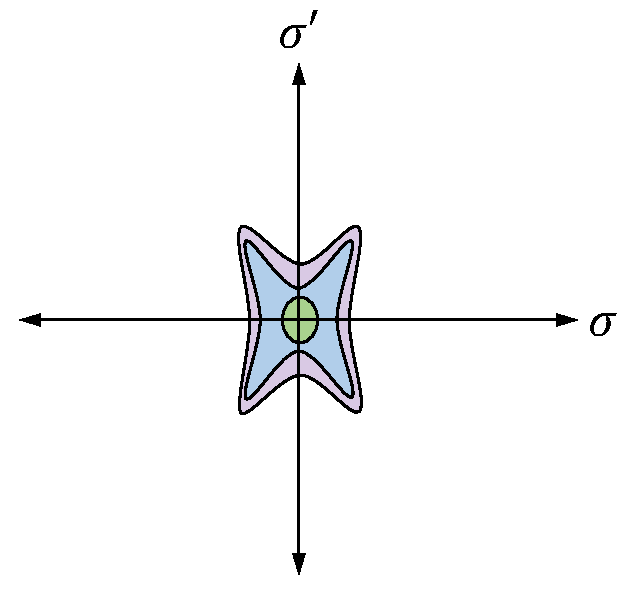
\includegraphics[height=3.1cm]{figures/ch02/e_smaller_u.pdf}}\\
        % \includegraphics[width=4cm]{figures/ch02/02_e_u_legend.pdf}\\



        
\end{figure}


\end{document}